\documentclass[
uplatex, a4j, dvipdfmx, 10pt, oneside
]{jsbook}
%
\usepackage{preamble}
\renewcommand{\thefootnote}{\fnsymbol{footnote}}
\title{関東夏ロボコン2020~講習会資料}
\author{関東春・夏ロボコン運営委員会\thanks{\href{mailto:kantouharurobo.official@gmail.com}{kantouharurobo.official@gmail.com}}}
\date{\today}

\begin{document}
\maketitle
\tableofcontents
\chapter{機械}
NHKロボコンにおいて機械の出来はそのチームの成績を大きく左右します. そのため, いかに性能を発揮できる機械を作れるかが鍵となります. 
\section{全体構成}\label{mecha:base}
NHKロボコンのロボットは大きく以下の3つの部位に分類できます.
\begin{itemize}
    \item 足回り
    \item 把持機構
    \item 投擲機構
\end{itemize}
このうち足回りはほとんどすべての競技に用いられる最も基本的な構造単位です. 把持機構や投擲機構は, 競技によっては直接用いることがない場合もありますが, どちらかの機構は必要になるでしょう. いずれにせよ, この3つの機構がロボットを設計する上で基礎的な事項となるので, しっかりとおさえておきましょう. 
\subsection{足回り}
ロボコンに用いられる足回りはいくつかの種類に分類できます. ここでは, それぞれの足回りについて特徴を紹介していきます.

\subsubsection{オムニホイール}
オムニホイールは, 図\ref{fig:omuni_round}に示すような主軸を中心とする回転部品の外周上に, 主軸方向に回転する複数の受動車輪がついた構造となっています. そのため, 主軸の回転方向には力を伝え, その主軸方向には力を逃がすようになります. この車輪を複数使用することで, 全方向に移動出来るロボットを作る事ができます. 一般に2次元平面上を動かす場合であれば, 2方向の向きと回転を制御できれば良いので, 3つ以上のオムニホイールを適切に配置すれば全方向に移動できるロボットを制作できます. 比較的簡単に全移動方向を実現でき制御難度も低いので, ロボコンにおいては多く用いられます. 

\begin{figure}[h]
  \centering
  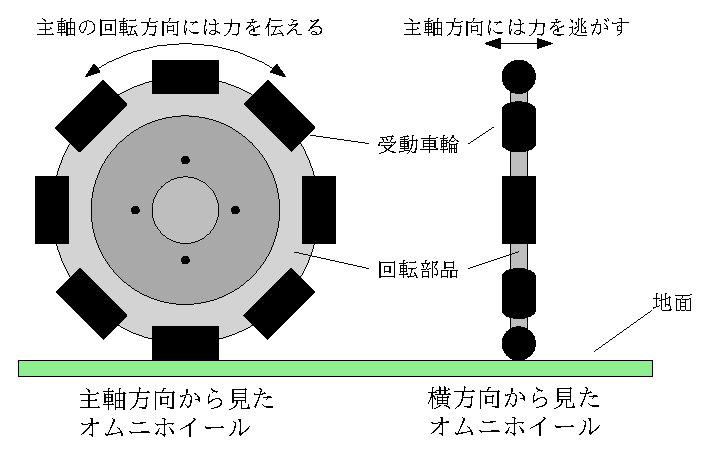
\includegraphics[width=10cm]{mecha/fig/omuni.eps}
  \caption{オムニホイールの構造}
  \label{fig:omuni_round}
\end{figure}

よく用いられる構成として, 図\ref{fig:3-omuni}のように3つのオムニホイールを正三角形の頂点に配置するものや, 図\ref{fig:4-omuni}4つのオムニホイールを正方形の頂点に配置するものがありますが, これ以外の構成でも3自由度が確保できるような構成であれば全方向移動するロボットを制作することができます. 
例えば図\ref{fig:4-omuni-po}のようにひし形の構成も可能です. しかし, 図\ref{fig:fiji}のように4つのオムニホイールを平行に並べてたような構成は1方向の移動と回転しか行えないため, 全方向移動は不可能です. このような場合は, 図\ref{fig:fiji_imp}のようにもう一方向に移動できる車輪を付け加えることで全方向移動が可能となります.

\begin{figure}[h]
 \begin{minipage}{0.5\hsize}
  \begin{center}
   \includegraphics[width=50mm]{mecha/fig/3-omuni.eps}
  \end{center}
  \caption{代表的な3輪オムニ配置}
  \label{fig:3-omuni}
 \end{minipage}
 \begin{minipage}{0.5\hsize}
  \begin{center}
   \includegraphics[width=50mm]{mecha/fig/4-omuni.eps}
  \end{center}
  \caption{代表的な4輪オムニ配置}
  \label{fig:4-omuni}
 \end{minipage}
\end{figure}

\begin{figure}[h]
  \centering
  \includegraphics[width=7cm]{mecha/fig/4-omuni-po.eps}
  \caption{変則的なオムニホイールの配置}
  \label{fig:4-omuni-po}
\end{figure}

\begin{figure}[h]
 \begin{minipage}{0.5\hsize}
  \begin{center}
   \includegraphics[width=50mm]{mecha/fig/fiji.eps}
  \end{center}
  \caption{オムニホイールが平行に4つ並んでいる機体}
  \label{fig:fiji}
 \end{minipage}
 \begin{minipage}{0.5\hsize}
  \begin{center}
   \includegraphics[width=50mm]{mecha/fig/fiji_imp.eps}
  \end{center}
  \caption{オムニホイールを付け足した例}
  \label{fig:fiji_imp}
 \end{minipage}
\end{figure}

注意点として, 全方向移動が出来るといっても, 形状によって方向によって速度の出しやすさ, トルクの出しやすさが異なります. ちなみに図\ref{fig:3-omuni},\ref{fig:4-omuni}のようなロボットの場合は最も速度及びトルクが出しやすいのは回転方向です. また, 接地点に関しても注意が必要です. 平面は3点で定まるので, 接地点が3つの場合は必ずすべての車輪が接地するため問題がないですが, 接地点が4つ以上ある場合, 地面の状況によってはすべての車輪が接地しない可能性があります. 接地しない車輪があると, その車輪は空回りをしてしまい, うまくロボットを制御出来なくなってしまうので, 必ずすべての車輪が接地するようにしなくてはいけません. ロボコンのフィールドは平坦であるので, 多くの場合は問題になりませんが, 足回りのフレームが過剰に硬いとうまく接地しないこともあります. 足回りのフレームはある程度柔らかいほうがこれらのトラブルを避けやすい
です. 
バネなどを用いて車輪を地面に押し付けてすべての車輪を接地させる方法もありますが, 機構が複雑になるほか, ばね定数等を適切に設定しないと振動の原因となってしまうのであまり推奨できません. 

\subsubsection{メカナムホイール}
メカナムホイールはオムニホイールと似ていますが, 図\ref{fig:mechanum_round}のように本体外周上についているローラーが, 本体に対して45$^{\circ}$傾いています. このホイールを図\ref{fig:mechanum}のように4つ配置することで, 全方向移動するロボットを制作できます. 

\begin{figure}[h]
  \centering
  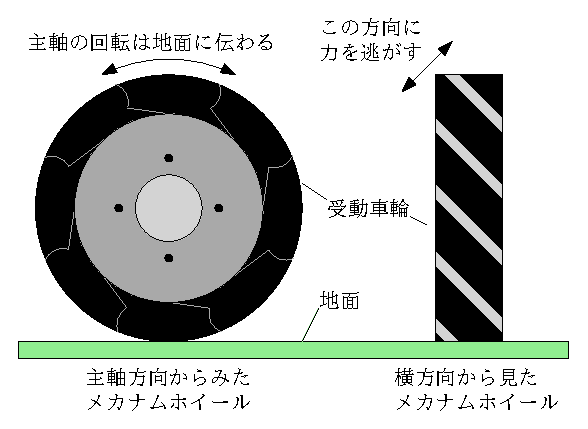
\includegraphics[width=10cm]{mecha/fig/mecanum.eps}
  \caption{メカナムホイールの構造}
  \label{fig:mechanum_round}
\end{figure}

\begin{figure}[h]
  \centering
  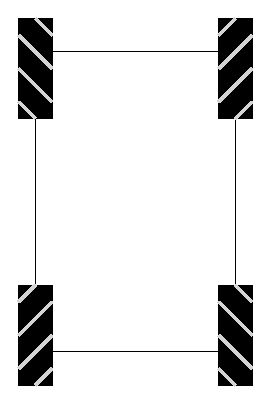
\includegraphics[width=5cm]{mecha/fig/fiji_mechanam.eps}
  \caption{メカナムホイールの配置}
  \label{fig:mechanum}
\end{figure}
基本的な事項はオムニホイールと同じですが, メカナムホイールは直進方向への運動性能が高いことが特徴です. その他, オムニホイールを用いるより足回りのフレームを組みやすいというメリットもあります. 

\subsubsection{独立二輪}
この足回りは, 通常の車輪を駆動輪として用います. 
図\ref{fig:sadou2}のように2つの駆動輪から成りますが, それだけでは機体を支えることができないのでキャスタなどを用います. この機体の特徴として, オムニホイールやメカナムホイールを用いたロボットと異なり, 全方向移動が出来ないことが挙げられます. 行きたい方向に行くには, その方向に機体の向きを変えてから移動する必要があります. このような機体は全方向移動出来る機体に比べて制御が難しくなります. 

\begin{figure}[h]
  \centering
  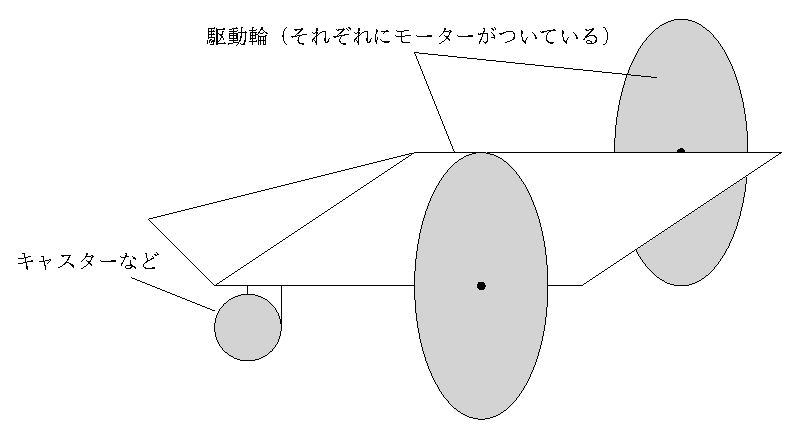
\includegraphics[width=10cm]{mecha/fig/sadou2.eps}
  \caption{代表的な独立二輪の配置}
  \label{fig:sadou2}
\end{figure}

オムニホイールやメカナムホイールと比べて車輪の制作や改良がしやすいため, より運動性能の高い機体を作りやすいというメリットがあります. また, 必要となるモーターが2つで済むため, 機体重量を軽量化できるという点もメリットです. 一方で機体の設計が難しいという問題があります. 独立二輪の機体で性能を発揮するためには駆動輪を必ず接地させる必要があります. 可能であればキャスターを1つにすれば接地の観点では最も良いですが, 安定性に劣ります. 一方でキャスターを2つ以上つけると安定性の観点では優れますが, うまく駆動輪が接地しない場合もあります. 
また, 急加速をした際にも機体が安定しているためには, 駆動輪が進行方向に対して中央にあるのが望ましいですが, その場合はキャスターを4つつけることとなります. この場合, より駆動輪の接地が難しくなるため, 設計段階からより注意が必要です. 

\subsubsection{独立四輪}
この足回りは長方形状の機体の各頂点に進行方向に並べられた4つの駆動輪から成ります. 
独立二輪と同じく, 車輪の制作や改良がしやすいというメリットがあるが, 旋回性能では大きく劣ります. 左右の車輪の回転速度の制御により, 若干の方向転換は可能でありますが, 基本的には直進性能を突き詰めたような足回りです. 一般的な競技には用いられないですが, 稀に存在するほとんど直進しか必要のない競技において用いられる場合があります. 

\subsubsection{独立ステアリング(swerve drive)}
通常のタイヤがそれぞれ方向転換出来るようになっていて, 進行方向に向けてタイヤの向きを変えることにより, 全方向への移動を実現します. こちらも通常のタイヤを用いるため, 車輪の制作や改良がしやすく, 独立二輪と同様運動性能の高い機体を作りやすいというメリットがあります. 

一方で, 車輪を二つの軸で回転させる必要があるため, 機構が複雑になり, 設計やメンテナンスが困難となるというデメリットがあります. 制御の難易度は機体の構成によって変わるので一概には言えないですが, ロボコンで多く用いられる車軸と旋回軸が同一平面上にあるタイプの機体は独立二輪と同程度の難易度です. 
ただし, これはすべての足回りにおいて言えることですが, より高い速度や加速度を出そうとするとより制御は難しくなります. 

\subsection{把持機構}
NHKロボコンにおいてフィールド上にあるオブジェクトを回収したり, オブジェクトを指定の位置に運搬するというのは非常に多く見られる課題です. 
そのため, オブジェクトの把持はロボコンにおいて非常に重要となります. 実際にオブジェクトを掴んで運搬するようなタスクがない競技であっても, オブジェクトを全く扱わない競技は稀であるため, 把持機構の考え方などは役に立つことがあります. 

尚, オブジェクトを運搬するだけならば引きずって運搬するという手段もあるという点は頭に入れておきましょう. ただしルールなどで禁止されている場合も多いですのでルールはよく確認しましょう. 

さて, ここではロボコンでオブジェクトの把持に用いられる機構を3つに分けて紹介します. 

\subsubsection{ハンドによる把持}
この手法は図\ref{fig:hand}に示すように2つもしくはそれ以上の方向からオブジェクトを挟むことで把持します. 
アクチュエータとしてはサーボモーターやエアシリンダなどを用いたものがロボコンでは多く見られます. 
把持する物体が同じであっても様々な種類や構造が考えられるため, ここでは個々のハンドを取り上げて解説はしません. 
インターネット等で調べれば様々なハンドを見つけることが出来るので, 各自調べて参考にしてください. 

\begin{figure}[h]
  \centering
  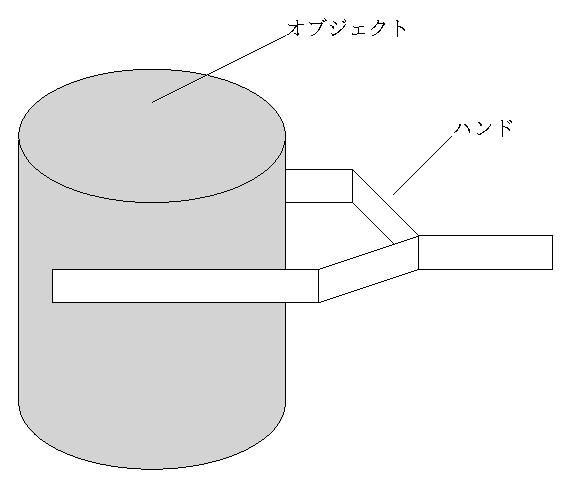
\includegraphics[width=7.5cm]{mecha/fig/hand.eps}
  \caption{ハンドによる把持の例}
  \label{fig:hand}
\end{figure}

ここで, ロボコンにおいて重要となるのはオブジェクトに対して最適化することです. 一般的に用いられるハンドはできるだけ多くの種類の物体を把持できるよう設計されていますが, ロボコンでは一つの種類のオブジェクトをつかめれば十分である場合が多いので, 目的のオブジェクトに特化したハンドを制作したほうが有利です. 
オブジェクトにふれる部分の形状や素材をオブジェクトに合うように設計, 改良して素早く, 正確にオブジェクトを把持できるようにすると, 競技を有利に進められる場合が多いです. 

メリットとしては確実にオブジェクトをつかめて信頼性が高いこと, 改良が施しやすいことなどが挙げられるが, オブジェクトが大きくなるとハンドも大きく, 重くなりやすいというデメリットもあります. 
\subsubsection{吸引パッドによる把持}
この手法は対象のオブジェクトを図\ref{fig:vacuum}のように吸引パッドなどを用いて吸着することで把持します. 
一般的には吸引パッドからポンプにつながっており, ポンプでオブジェクトと吸引パッドの間の空気を抜くことでオブジェクトを把持します. 
ロボコンではポンプではなくダクテッドファンを用いてこの吸引を行う場合もあります. 

\begin{figure}[h]
  \centering
  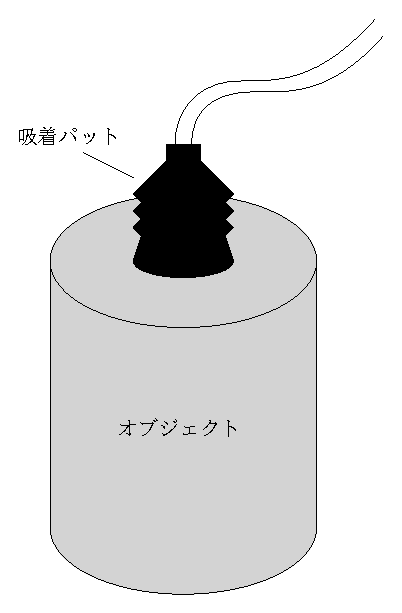
\includegraphics[width=5cm]{mecha/fig/vacuum.eps}
  \caption{吸引パッドによる把持の例}
  \label{fig:vacuum}
\end{figure}

吸引パッドを用いた把持方法は産業界でも多く用いられており, 様々な種類の吸着パッドが各メーカーから販売されています. オブジェクトによって適した吸着パッドは異なるのでメーカーの説明などを参考に適した吸着パッドを選ぶことが重要となります. 

メリットとしてはオブジェクトに吸引パッドがふれるだけで把持が行えるため機構が簡単になり, 様々なオブジェクトに対応できるという点があります. 
一方デメリットとして重いオブジェクトを把持することに適していないことや, オブジェクトの表面性状によっては使用できないこともある点です. 特にオブジェクトの表面性状に関しては注意が必要で, 練習用のオブジェクトでは把持できたが本番のオブジェクトでは把持できなかったという事象も起こりやすいので, 採用の際には十分な調査, 検証をおすすめします. 
\subsubsection{オブジェクトの形状に合わせた把持}
この手法は使用できるとは限りませんが, 使用できれば大きなメリットとなる可能性のある方法です. 
例えば図\ref{fig:advance}のように穴の空いているオブジェクトであれば棒状をアームを差し込んで引っ掛けて把持したり, 引っかかりうる部位のあるオブジェクトであれば鉤爪状のものを引っ掛けて把持したりすることが出来ます. 

\begin{figure}[h]
 \begin{minipage}{0.5\hsize}
  \begin{center}
   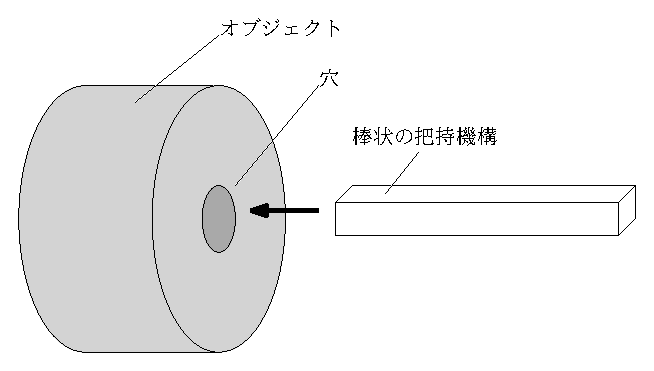
\includegraphics[width=75mm]{mecha/fig/hole.eps}
  \end{center}
 \end{minipage}
 \begin{minipage}{0.5\hsize}
  \begin{center}
   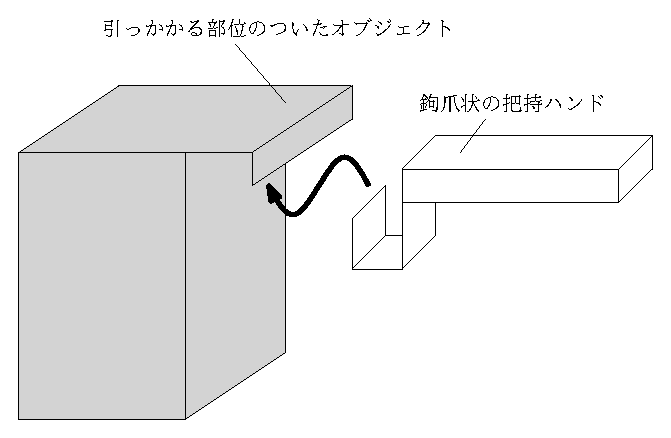
\includegraphics[width=75mm]{mecha/fig/kagi.eps}
  \end{center}
 \end{minipage}
 \caption{オブジェクトの形状を利用した把持の例}
 \label{fig:advance}
\end{figure}

これらの方法は使用するオブジェクトの形状や特性に大きく依存しており, このような形状であれば使用できる, 使用したほうが有利となる, という明確な答えはありません. 
しかしながら上記のハンドや吸着パッドを用いる方法よりも簡単に把持できたり素早く把持出来たりする場合は上記2つの手法に対して大きなアドバンテージとなります. ロボコンの「アイディアで魅せられる」部分でもあるので, 使用するオブジェクトをよく分析して上記2つの方法でない何か良い把持方法がないか考えることもアイディア会議の段階では大切にしましょう.
\subsection{投擲機構}
投擲は競技によっては全く必要のない場合もある一方で, 近年のNHKロボコンでは投擲が必要なルールが増えてきています. 投擲は難しい部分でもあり, 差が出やすい部分でもあるので設計段階から重要となる部分です. 

投擲の際に詰まるポイントとしてよくあるのは, 飛距離が出ないことと正確性が確保出来ないことです. 競技によっては正確性が問題とならない場合もあるものの, 多くの場合は目標の位置を通過もしくは着地するようにオブジェクトを投擲する必要があり, 毎回正確に目標位置に投擲ができなくてはいけません. 
飛距離に関してはオブジェクトに対して適切なエネルギーを与える必要がありますが, 機械の強度が不足していたりアクチュエーターの選定が不十分であると必要なエネルギーをオブジェクトに与えることが出来ません. 正確性に関しては投擲機構自体に正確性が低い場合もありますが, それ以外の要素も加わってくるので注意が必要となります. 代表的なものが足回りで, 毎回同じ位置に停止できるか, 角度にずれはないかなどが投擲の結果を左右します. この問題には足回りをどの程度ずれているかを正確に計測して目標の位置に正確に制御する技術等で対処することが多いですが, 壁などを利用してロボットを押し当てて位置や向きを修正するという方法もあります. 
他にも, オブジェクトと投擲機構によってはそれらの性質などが投擲結果の正確性に関わってくることもあります. このあたりはオブジェクトの形状や特性によっても変わってくるので実験を繰り返してデーターを集め, 原因を突き止めて修正していくことが重要となります. 

さて, 投擲に関してはオブジェクトの形状や重量などによって多数の方法が考えられますが, 今回は比較的多くのオブジェクトに適応できる例に絞って紹介します. 
\subsubsection{ベルト・ローラー型}
図\ref{fig:roller}に示すようにオブジェクトに2方向もしくはそれ以上の方向から回転するベルトもしくはローラーを押し当ててオブジェクトを加速, 射出します. 野球などのピッチングマシーンでも同様の仕組みが用いられています. ローラーやベルトによって与えるエネルギーによってオブジェクトを投擲するため, ローラーやベルトからスムーズにエネルギーを伝えられるかが鍵となります. 
ローラーやベルトがオブジェクトに対して滑ってしまうとエネルギーの伝達がスムーズに行かないので, ローラーやベルトの性能が重要となってきます. 

\begin{figure}[h]
  \centering
  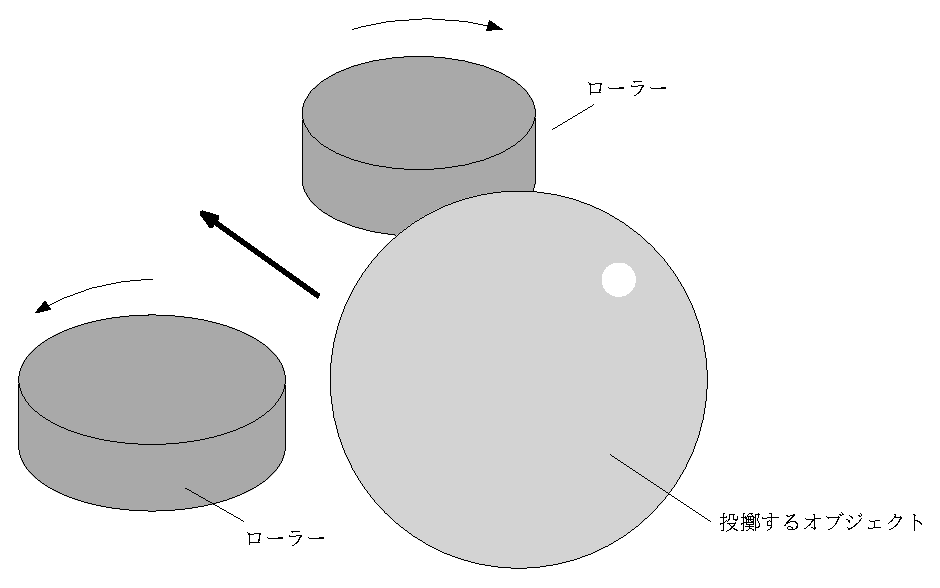
\includegraphics[width=10cm]{mecha/fig/roller.eps}
  \caption{ベルト・ローラー型の投擲機構}
  \label{fig:roller}
\end{figure}

比較的簡単に制作でき, オブジェクトの装填から射出までがスムーズであるというメリットがありますが, 柔らかいオブジェクトの投擲には向いていません. 
\subsubsection{直動カタパルト型}
図\ref{fig:cataput}のように直線上に高速に動く台などの上に投擲したいオブジェクトをセットし, 台とオブジェクトを加速した後, オブジェクトを台から分離することで投擲を行います. 
直動機構の性質上, 加速距離が限られるため, 非常に素早く加減速を行う必要があります. 
そのため機械的な負荷が大きく, アクチュエーターの選定や機構の設計などには注意が必要です. 

\begin{figure}[h]
  \centering
  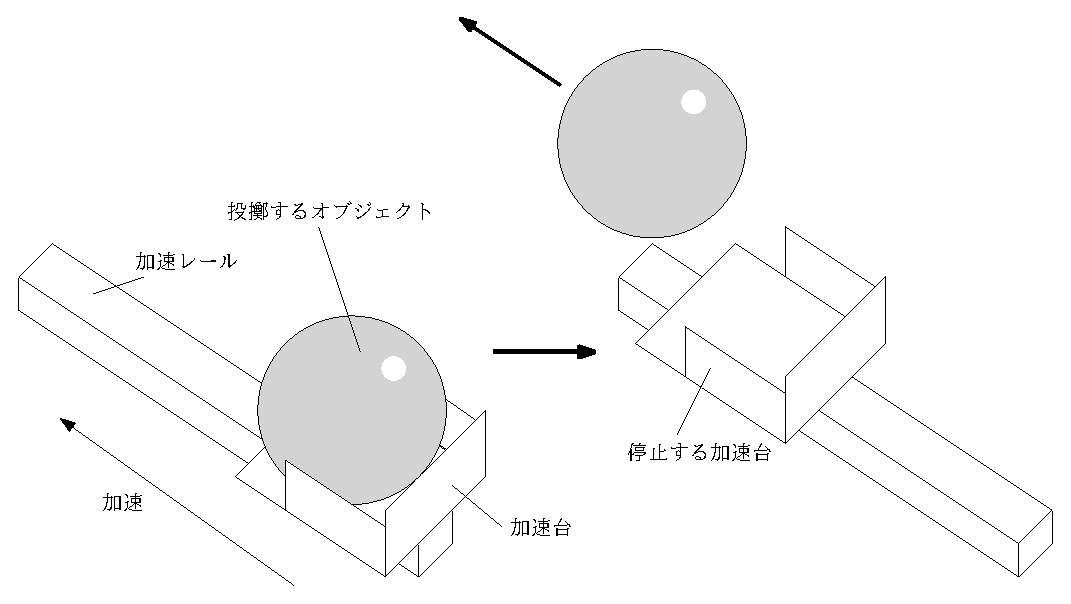
\includegraphics[width=15cm]{mecha/fig/catapult.eps}
  \caption{直動カタパルト型の投擲機構}
  \label{fig:cataput}
\end{figure}

機構自体の仕組みは単純であるものの, 競技によってはオブジェクトを装填が困難となる事があります. 
\subsubsection{回転アーム型}
図\ref{fig:rotate}のように回転するアームに投擲したいオブジェクトをセットし, 回転して加速させて後, 適切な位置でリリースすることで投擲する方法です. アームが複数回回転できるように設計することで加速時間を長く取ることができ, 機械的な負荷が小さいというメリットがあります. 一方であまり大きなものを投擲するのには向かない. また, 投擲に時間がかかることもデメリットとなるでしょう. オブジェクトをセットしたりリリースする機構の設計も重要となるため, 注意するようにしましょう. 

\begin{figure}[h]
  \centering
  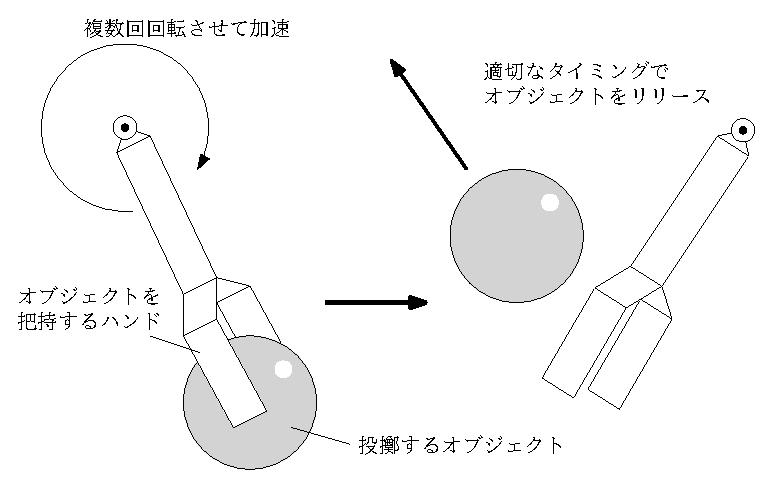
\includegraphics[width=12.5cm]{mecha/fig/rotate.eps}
  \caption{回転アーム型の射出機構}
  \label{fig:rotate}
\end{figure}

尚, このアームを1回転未満で運用する場合は急加速, 急減速を必要とするため, 直動カタパルト型の機構特徴を持つのでそちらを参照してください.
\section{基本的な設計指針}
第\ref{mecha:base}章ではロボットの全体構成について説明しました. では実際にロボットを設計していく際にどのような手順を踏んでいけばよいか, 順を追って解説していきます. 
\subsection{アイデアの収集}
どのようなロボットを作る場合においてもアイデアが非常に重要で, これをなくしてロボットを作り始める事はできません. 要するに作り始める前に機体及びその機構のイメージをしっかりと定めなくてはいけません. 
そしてこれは機械においては非常に重要となります. 機械はどうしても制作に時間がかかる上に改良で見込める性能向上は限られているからです. 制作したロボットが求める性能が出なかった場合はまた1から作り直すことが必要となってしまいます. そのため, 1年で結果を出すことを求められるNHKロボコンにおいては良いアイデアを出来るだけ早く得ることが非常に重要となります.

さて, ではどのようにアイデアを得るかが問題となるでしょう. 行いたい動作を達成する機械をどのように構成するかは設計者によって個性が出る部分であり, 同時に性能の差も付きやすい部分です. 行いたい動作の発想自体は悪くなかったとしても, それを実現するためのアイデアが浮かばなければ意味がありません. 
ここで, あまり経験がない人ほど考え込んでしまう場合が多いです. もちろん, 考えることは悪いことではないですが残念ながら天才でもない限りいきなりアイディアが浮かぶということはありません. 
ここで, 実際に作ってみるなどして自分で手を動かしてみることが大事というのが世の中ではよく言われます. これは非常に正しいですし, 最終的にはそうやって得られるアイデアも非常に多いのですが, その前に少しやったほうが良いことがあります. それがアイデア収集です. というのも前述したとおり機械は制作に時間がかかります. 手を動かしてみて作った後にそれから得られた知見をもとに作り直すには限度があります. あと5年位あればもっと良いものが出来ていたのに……という事になりかねません. この作り直しを減らせる可能性があるのが事前のアイデア収集です.

NHKロボコンではルールが毎年変わるために過去のアイデアが全くそのまま用いられるわけではありません. しかしながら, 小さな機構単位であれば役に立つことは多くあります. そのため, 過去のロボコンに出場したロボットを分析してアイデアを収集することはまず行うべきでしょう. 自分のやりたい動作に近い動きをしている部分はないか, どのようにその動作を達成しているか, それは自分たちには可能かを調べて参考にすると良いです. 

また, 世の中に存在する機構からもアイデアを得ることは出来ます. 身の回りに面白い動きをしているものや, 役に立ちそうな機構があればそれを応用することも出来るでしょう. ただし, スケールの違うものはそのまま適応出来ないこともあるのでその点は留意しておく必要があります. 

\subsection{機構の選定}
ある程度アイデアを集めることができたら, 次に必要なのはその取捨選択です. 望ましいのは考えられうるすべての機構を実際に作ってみてその性能を評価することですが, 資金も時間も限られるNHKロボコンにおいてこれは現実的ではない場合もあります. ではこれに対する対応策を考えてみましょう.

よくあるのは勝負を左右する重要な機構においては複数種類作って実験を行い, その性能を評価するが, それ以外の機構については最もうまくいきそうな機構, 場合によっては設計者の好みの機構を採用するという方式です. 
メリットとしてはその競技に最も適していそうな機構を採用することができる点です. 
一方で人や資金, 時間が豊富でないと出来なかったり, 中途半端に終わってしまうことがあるという点はそのような資源が豊富でないチームにおいてはデメリットです. 機構を評価してどの機構に決定するかに長い時間をかけてしまい, 肝心のロボット制作の時間が大きく減ってしまったという話もよく聞かれます. 
また, どのように評価するかを定めておかないと機構の決定が難航する点にも注意しましょう. 評価軸がブレブレであったり, 特定の個人の主観が強く反映された評価軸は適した機構を選定できないばかりか, その後のチーム運営にも大きな悪影響ともなりうるので注意が必要です. 

勝負を左右するような機構も最初から1つの機構に絞ってしまい, それを突き詰めるという方式もあります. 
これはどの機構に絞るかによって最終的なロボットの性能が決定してしまうというデメリットがありますが, チームの人数や資金, 活動時間に制約があるチームではこちらの方式が適していることもあります. 
というのも, NHKロボコンはどのチームも開発期間が1年で, 機構の最適化が完全に行いきれないためです. そのため, あまりその競技やタスクに適していないような機構であっても, しっかり開発できていれば十分に勝負出来ます. 実際に, 機構は全く違うがほとんど同じ成績を出すロボットも毎年多く見られます. これは優勝するようなレベルのロボットに関しても例外ではありません.
ただし, どのような機構であってもしっかり開発すれば優勝を目指せるというわけではありません. ある程度の性能を発揮できる機構であることが前提条件です. そのために, 採用しようとする前に候補となる各機構の調査及び分析を行うことは非常に重要となります. 過去の使用例や, その機構を使用した人の経験談, 過去にその機構を採用した理由や開発経緯など, 様々な観点から情報を集めて判断に役立てると良いでしょう. 

\subsection{アクチュエータの検討}
実際にどのような機構を採用するか決定する前から, 各機構に使用しうるアクチュエータに関してはよく検討する必要があることもあるため, 前項の機構の選定と順番が前後します. 

実際に作りたい機構にどのアクチュエータを使用するかは制御する側にも大きく影響があるためアクチュエータを決定する際には制御担当者とよく話し合う必要があります. 決して機械側の都合だけで決定せず, 制御側の都合も考慮してお互いが納得するように決定するようにしましょう. 

さて, 機械的な観点ではアクチュエータは回転する形で動力を取り出せるものと, 直動の形で動力を取り出せるものの2種類があります. 回転することで動く機構に関しては回転する形で動力を取り出せるアクチュエータ, 直動することで動く機構は直動の形で動力を取り出せるアクチュエータが望ましいですが, 直動と回転は変換が可能なので, あまり大きな問題にはなりません. 直動と回転で違いがあるとすれば減速, 増速のしやすさです. 一般に直動するタイプの機構は大きな減速や増速は行いにくいです. そのため, 必要なトルクや速度を出せるアクチュエータがないと設計が困難となります. 
一方で回転するタイプのアクチュエータはギアなどを使用すれば簡単に増速や減速が行えます. そのため必要なトルクや速度をそのまま出力できるアクチュエータがなかったとしても, 減速機で調整することで必要なトルクや速度を得ることが出来ます. 

アクチュエータの分類として他に, 電気エネルギーで動くか空圧で動くかという分類も考えられます. 例外はあるものの, 電気で動くアクチュエータは各種モーターなど回転する形で動力を取り出せるものが多いです. 空圧で動くアクチュエータはエアシリンダーなど, 直動の形で動力を取り出せるものが多いです. 
電動のアクチュエータを使用するか空圧のアクチュエータを使用するかは制御側の都合も大きく関わるので機械の都合だけで決定はできませんが, 機械側の観点として, 空圧は多くの体積が必要であることを頭に入れておきましょう. 電動アクチュエータは多くの場合バッテリーを1個か2個搭載しておけば試合時間を乗り切ることが出来ますが, 空圧の場合はそうとも限りません. 使用する量が多い場合は大量の空圧タンクを必要とします. NHKロボコンでは空圧タンクとしてペットボトルが用いられる事が多いですが, 使用する空気の量が多いとこのペットボトルを10本以上搭載することが必要な場合もあります. また, 使用すればするほど出力が低下していくことにも気をつけましょう. 出力が一定であることが必要な機構などでは使用に向きません. 
また, 空圧は危険であることもよく頭に入れておく必要があります. そのため, 空圧タンクにダメージが加わらないような設計や, 空圧タンクを守る構造及びスペースも確保しなくてはいけません. これらのスペースについてもアクチュエータを考えるときに気を配るようにしましょう. 
\subsection{その他調整が必要な部位}
ここまでは個々の機構についての設計方針について述べましたが, ロボット全体のバランスを考えて調整が必要な場合があります. 特に, オブジェクトを取得してから投擲したりセットしたりする過程でオブジェクトが複数の機構を経由する場合はそれぞれの機構との調整が欠かせません. お互いの機構が干渉する可能性やオブジェクトをどの向きで受け渡すかなどはよく考えるべきでしょう. また, 機構単体で見ると良い性能であっても, 両方とも搭載すると展開制限を超えてしまうなどの場合もあります. このような場合, そのまま両方とも採用することは出来ないので全体の構成を決める際には注意しましょう. 
他にも, ロボットのどの位置に機構を取り付けるかによっても全体の性能が変わってきます. とりあえず機構さえ搭載しておけばよいというものではないので, それぞれの機構がロボットのどの位置に搭載する必要があるのか, 他にその位置に搭載する必要のある機構がないかも考えつつ設計すると良いでしょう. 

\section{実際に機械を設計及び制作していく際の留意事項}
ここまでは, 各機構の決定及び設計を主眼に解説してきましたが, 実際にロボット全体の設計及び制作を行っていく際には他にも留意すべき事項があります. 
\subsection{回路の搭載}
多くのロボットでは回路がないと動くことは出来ません. 回路は機械を設計する人にとってはあまり馴染みがないものかも知れませんが, 最低限どの程度の大きさがあって, どのように搭載するか, どの位置に設置する必要があるかは知っておきましょう. そして, 回路を載せるスペースを忘れずに設けるようにしましょう. ここでの回路にはセンサーなども含みます. 制御する人からセンサーを搭載してほしいと言われた場合は, どこに搭載するべきか, どのように搭載するかをよく話し合って決定し, 搭載するようにしましょう.
また, 回路だけでなく, モーターやセンサーからはケーブルが出ていることも忘れてはいけません. ケーブルをどこを通すか, ケーブルが機構の邪魔にならないかなども設計の際に頭の片隅には置いておくようにしましょう. 
\subsection{重量}
重量はロボコンにおいては常に付いて回る課題です. NHKロボコンは重量制限が厳しい傾向があり, 注意していないと制限を超えてしまうことも多々あります. 各機構を設計する段階からどの程度の重量を目指すべきか, 機構ごとに大まかな目安を付けて設計していくようにすると良いでしょう. 
例えば, 重量制限が20kgのロボットを設計しようとしたときには, 足回りの目標重量が10kg, アームが2kg, 投擲機構が3kg, 回路(バッテリー含む)が3kg, ペットボトルなど空圧機器が1kg, 余裕が1kgで合計20kgといった具合です. 
これらの目標を達成できるか, 達成できそうにないならどこの重量を削るかを常に考えながら設計, 制作をするようにすると良いでしょう. 
\subsection{各機構の統合}
多くの場合, 1つのロボットを設計する際に, 機構ごとに担当を分担し, それぞれの担当者が設計した後に統合するという方法をとります. この場合, 各機構の設計が終了したあとにそれぞれの機構を統合しようとすると, うまく統合できなかったり統合に多くの時間がかかってしまったりする場合がしばしばあります. 
このような事態を避けるため, 設計を始める前に各機構の大きさや接続方法を可能な限りしっかりと定めておくようにしましょう. 
また, 設計中にもお互いの連携を欠かさず, 想定外のサイズ変更や要件変更などは常に共有する習慣をつけましょう. 
しっかりと連携をとっておけば, 最終的に統合して1つのロボットにするときにも想定外の事態が発生せず, スムーズに統合することができます. 複数人で1つのロボットを作っているという意識を忘れないようにしましょう. 
\subsection{納期}
実際に制作していく際には, 納期は常についてまわる問題です. 機械は部品が届かないと制作が出来ません. 
材料はどこから購入するのか, その場合の納期はどのくらいかは頭に入れて行動するようにしましょう. 例えば, 納期に1週間かかることがわかっていて使う予定のある部品は, 組み立てが始まる1週間より前に発注するなど, 全体として制作が滞るような事のないように気をつけましょう. 
また, 加工にどのくらいの時間がかかるかも頭に入れておく必要があります. 自分たちの使える加工設備の処理能力などからどのくらい加工に時間がかかるかは理解しておくようにしましょう. これらの時間は, 伸びることはあっても, 縮まることはほとんどないということも気をつけなくてはいけません. さらに, 回路の搭載や制御の時間などは機械の設計や制作には関係ありませんが, 最終的なロボットの完成には欠かせないものとなっています. 制御にどの程度の時間が必要かよく話し合い, 制御の時間を圧迫しないように計画を持って制作に行うようにしましょう. 
納期に遅れそうなときは直ちにそのことをチーム全体に共有し, 計画の見直しを行うようにしましょう. 計画の見直しを行わないとなし崩し的に予定が延びていきます. 機械は納期の短縮が難しいことを頭に入れ, 無理のない計画, こまめな見直しを忘れないようにしましょう. 
\chapter{回路}

NHKロボコンに出場するロボットにおいて,回路は主に図~\ref{fig:circuit_overview}に示すような範囲を担当します.図~\ref{fig:circuit_overview}~(a)にあるように,ロボットが1)~なんらかのセンサ入力を受け取り,2)~それを処理して,3)~なんらかの運動を出力するシステムであると考えたとき,回路が提供する主な機能としては a)~物理量を計算機で扱える形に処理すること,b)~計算資源を提供すること,c)~アクチュエータを駆動すること,の3点があげられます.
本章ではこの3つの機能について,ロボットの回路構成を決定する上で必要となる事項をそれぞれ解説します.
この資料は様々な回路要素を比較し,回路の視点からロボットの構成を検討することができるようになることを目的としています.
このため,各回路の動作原理等の詳細については省略いたします.
実際に実装する際には,本資料も参考にしつつ自習していただければ幸いです.

\begin{figure}[h]
  \centering
  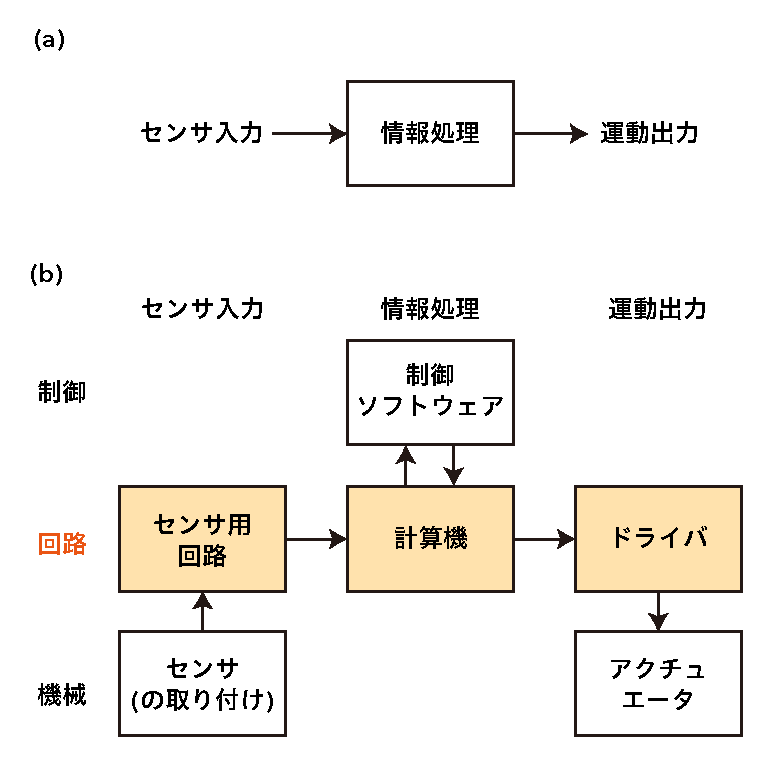
\includegraphics[width=10cm]{circuit/fig/1_circuit_overview.pdf}
  \caption{回路の視点で見たロボットの構成.(a) 大まかな構成. (b) 制御,回路,機械のレイヤに分類した場合の構成.オレンジの部分が回路の担当部分を示している.図中の矢印は主な処理の流れを表す.}
  \label{fig:circuit_overview}
\end{figure}


\section{計算機}

まず初めに,ロボットの回路構成の決定に大きく影響する計算機について説明していきます.

\subsection{計算機の種類}

NHKロボコンで用いる計算機は,図~\ref{fig:computers}のように分類でき,それぞれロボットに合わせて搭載するものを選びます.

マイコンは,計算速度は速くないものの,安価であることや入出力ピンが多数あり多くのセンサやアクチュエータを制御できること,ハードウェアの細かな制御が行いやすいといった利点があります.
ロボコンではセンサやモータなどのハードウェアを扱うため,マイコンを使用する場面が多くあります.

シングルボードコンピュータは,PCとマイコンの中間的な存在です.PCほどではないが高速なプロセッサを搭載しているため,LinuxなどのOSが動作します.
しかし,PCとは異なり入出力ピンを備えていて,ハードウェアを制御することも可能です.
価格も1万円以下で買えるなど,非常に入手しやすいものとなっています.
計算量の多い制御を行いたい場合や,USBやEthernetで通信して用いるセンサ(カメラやLiDARなど)を用いる場合,ロボットをインターネットに接続したい場合などに便利です.

そして,シングルボードコンピュータよりもさらに大きな計算資源が要求される場合は,PCを使います.
計算資源が必要である場合の他に,タブレットPCをロボットの状態を示すディスプレイとして兼用することを意図してPCをロボットに搭載するチームもいます.

以上,価格・速度や入出力端子の観点で比較をしてきましたが,この他に,計算機を選定する場合の観点としてリアルタイム性というものがあります.リアルタイム性とは,計算が決められた時間以内に完了するかどうかという性質のことを指します.
ロボットの制御では,センサを読み取り出力を変更するということを一定周期で行う必要があるため,リアルタイム性が要求されることが多いです.
計算が終了するまでの時間が保証されていないと,例えばセンサはフェンスを捉えていたのにモータの出力を変更する処理が間に合わずフェンスに衝突してしまうなどの事故が発生してしまいます.
リアルタイム性を確保するための方法としては,リアルタイムOSを用いることや,OSがない状態でハードウェアのタイマー(マイコンに内蔵されている)を用いることなどがあります.
PCやシングルボードコンピュータを一般的なOSで用いる場合は,リアルタイム性を確保することを意図してシステムが作られていないため注意が必要です.

\begin{figure}[h]
  \centering
  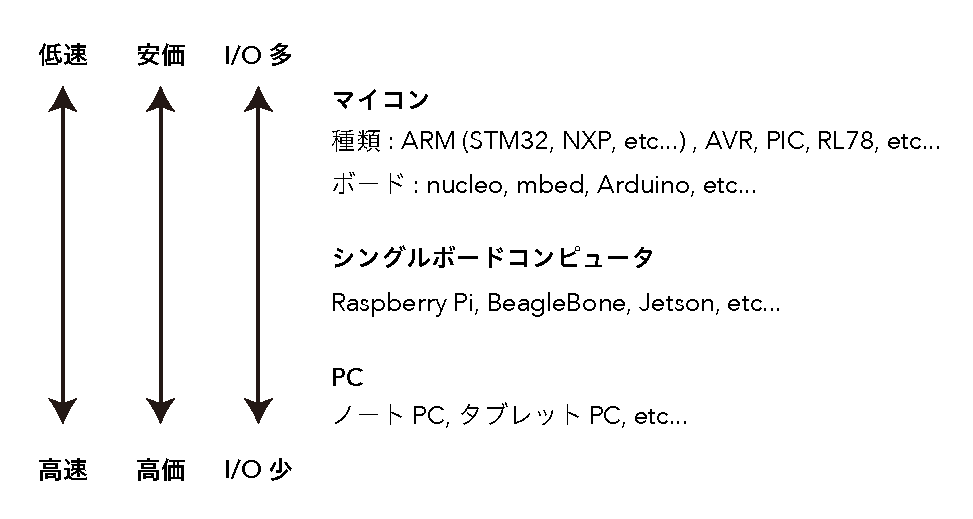
\includegraphics[width=10cm]{circuit/fig/2_computers.pdf}
  \caption{計算機の種類.}
  \label{fig:computers}
\end{figure}


\subsection{計算機まわりの回路構成}

NHKロボコンで用いる代表的な回路構成の例を図~\ref{fig:circuit_system_configuration}に示します.ロボット全体の動作を制御するソフトウェアを動かす回路として,メインボードなどと呼ばれる回路がロボットに搭載されることが多いです.メインボードに搭載されたマイコンを中心にして,ロボットの制御が行われていきます.以降,このメインボードを中心に回路の構成を説明していきます.

最も計算機の数が少ないのはマイコンを1つのみ搭載する構成です.この場合,メインボードのマイコンから直接デジタル信号またはアナログ信号を入出力してロボット全体を制御します.続いて,モータドライバやセンサ用の回路などそれぞれの回路にも1つずつマイコンを搭載するような構成もあり得ます.この場合,メインボードのマイコンは各デバイスのマイコンとシリアル通信して制御を行います.これに加えて,PCが搭載される場合もあり,メインボードのマイコンとUSBシリアル変換ICを介すなどして通信し制御を行います.メインボードと書かれている部分には,Arduinoのようなボードを用いたり,シングルボードコンピュータを用いたりすることもできます.

マイコンが1つのみの構成の利点としては,以下のような点が挙げられます.

\begin{itemize}
    \item 安価に製作できる
    \item 通信機能の開発を行わなくて良い
\end{itemize}

これらの特徴があるため,初めてロボットを製作する初心者でも扱いやすいです.一方,以下のような欠点が存在します.

\begin{itemize}
    \item ロボットに合わせてメインボードを作り替える必要がある.同じ回路を使い回すことが難しい.
    \item マイコンのピン数に限りがあるため,多くのモータやセンサを用いることが難しい.
\end{itemize}

マイコンが1つのみの構成では以上のような欠点があり,ロボットの規模が大きくなると限界を迎えます.この限界を突破するために,各デバイスにそれぞれマイコンを搭載することも多いです.図~\ref{fig:circuit_system_configuration}ではセンサ,モータドライバと区別して図示していますが,モータドライバにセンサが接続されていてモータ制御を行う構成もよくあります.このような構成ができることも,マイコンを複数搭載することの利点です.この構成の利点としては以下のような点が挙げられます.一方欠点としては,回路にかかる費用が上がることや通信機能を開発しなければならない点が挙げられます.

\begin{itemize}
    \item モジュール化して同じ回路を使いまわしやすい.通信するデータのフォーマットをうまく設計すればブラックボックスとして扱うこともできる.複数人での開発もやりやすくなる.
    \item 通信量が多すぎない限り,基板の枚数を増やすことで機能を増やせる
    \item 1つのモータに対して1つのマイコン,と言うような使い方ができるため制御周期を短くしやすい.制御の章で説明されるマイナーループを各デバイスのマイコンで高速に回し,メジャーループをメインボードと通信しつつやや長い制御周期で回すという使い方ができる.
\end{itemize}

以上に加えて,高速な計算資源が必要な場合や,カメラ等動作させるために必要なソフトウェア(ドライバ等)がPC用に提供されておりPCを搭載すれば簡単に利用できる場合など,PCやシングルボードコンピュータを追加で搭載することがあります.
これらの計算機上でリアルタイムOSを動作させることも可能であるが,リアルタイムでないLinuxなどを用いる場合はメインボードとの通信のタイミングなどに注意して開発を行う必要がある
(回路担当としては通信ができるようにハードウェアを用意するのみで,どちらかと言うとプログラムを開発する人が注意する必要がある).


\begin{figure}[h]
  \centering
  \includegraphics[width=10cm]{circuit/fig/3_systemconfiguration.pdf}
  \caption{回路の構成}
  \label{fig:circuit_system_configuration}
\end{figure}

\section{センサ}

続いて,センサについて解説します.NHKロボコンでは多くの場合センサデバイスは購入してきて使います.従って,回路担当は購入したセンサデバイスを適切な条件で動作させ,出力を処理して制御に用いることができるようにするための作業を担当します.本章では,それぞれのセンサを用いるために必要な回路について説明します.

\subsection{センサの種類}

センサには様々な種類があるが,ロボコンでしばしば用いるものとして次のセンサが挙げられます.以下,それぞれについて簡単に性質を述べた後,それぞれに必要な回路について説明します.

\begin{itemize}
    \item スイッチ
    \item 距離センサ
    \item ロータリーエンコーダ・ポテンショメータ
    \item 加速度センサ・ジャイロセンサ
    \item ラインセンサ
\end{itemize}

\subsubsection{スイッチ}

まず,最も単純なセンサとしてスイッチが挙げられます.スイッチは反応しているか,していないかの2値を返します.回路的に言えば,スイッチは電圧が高い状態か,低い状態かの2値を出力します.

スイッチには様々な種類があります.まず,機械的に金属の接点が接触したり離れたりすることによって出力が決まるスイッチとしては,コントローラなどに用いるスイッチや,リミットスイッチ(マイクロスイッチ)(Fig.~\ref{fig:circuit_switch})と呼ばれる物体をぶつけて反応させるタイプの小さなスイッチがあります.
リミットスイッチは機構の稼動範囲の両端に設置して機構を止める位置を検出する用途や,オブジェクトへの接触を検知する用途などに用います.

一方,非接触型のスイッチとして,光を利用したフォトリフレクタ(Fig.~\ref{fig:circuit_switch})や光電センサなどがあります.
これらは照射した光がフォトセンサに当たるか当たらないかによって物体の有無を検出するものです.
ものによっては反応距離を変えることができる,スイッチから少し離れた位置にあるものを検出することも可能です.
また非接触であるため壊れにくいです.
用途としては機械式スイッチと同様に機構の稼動範囲を決めたり,ロボット間で連携をする際に相手のロボットの接近を検出する用途に使います.
非接触のスイッチとしてはこの他に,磁石が近づくと反応するタイプのリードスイッチもあります.

\begin{figure}[h]
  \centering
  \includegraphics[width=10cm]{circuit/fig/switch.png}
  \caption{スイッチ}
  \label{fig:circuit_switch}
\end{figure}

\subsubsection{距離センサ}

フェンスやオブジェクトまでの距離を測定したい場合は距離センサを用います.自動ロボットではロボットの自己位置を推定するために用いるセンサです.距離センサとしては,超音波を用いるもの,赤外線を用いるもの(PSD距離センサ, Fig.~\ref{fig:circuit_psd}),レーザーを用いるもの(ToF方式の距離センサなど)などがあります.
出力方式には様々なものがあり,アナログ出力をするものや,シリアル通信で読み出すものなどがあります.
この他に,LiDARという2次元または3次元の距離情報を一気に読み取ることのできるセンサもあります.LiDARはPCやシングルボードコンピュータにUSBやEthernet経由でつないで用いることが多いです.

\begin{figure}[h]
  \centering
  \includegraphics[width=10cm]{circuit/fig/psd.png}
  \caption{赤外線距離センサ}
  \label{fig:circuit_psd}
\end{figure}

\subsubsection{ロータリーエンコーダ・ポテンショメータ}

ロータリーエンコーダやポテンショメータ(Fig.~\ref{fig:circuit_enc})は回転角度を計測するセンサです.センサに回転軸がついていて,その軸が回された角度が分かります.
ロータリーエンコーダには,相対的な回転角度が計測できる(何度回ったか,という情報がわかるが,回転しなければ出力がない)インクリメンタル型と,絶対角度が計測できる(出力値が0度になる原点が決められていて,そこから何度回った位置にいるのかがわかる)アブソリュート型があります.ロータリーエンコーダは軸の回転に合わせて円盤が回転し光が遮られたり透過したりして回転角度を計測する光学式のものや,磁界の変化を計測して回転角度を調べる磁気式のものなどがあります.ポテンショメータは回転角度によって抵抗値が変化する,いわゆるボリュームのことです.ポテンショメータは基本的に絶対角度を出力します.
これらの回転角度センサの用途は主に2つあります.1つ目はモータに取り付けてモータ制御のためのセンサとして使うことです.モータが何度回転したかということがわかるため,位置制御や速度制御などが可能になります.2つ目は,ロボットの自己位置推定のために用いるもの(いわゆる,接地エンコーダ)です.ロボットがフィールド上のどこにいるかを調べるために,車輪を床に接地させ,その車輪の回転角度をもとにロボットが進んだ距離を計測します.

ロータリーエンコーダの出力は,一定角度回転するごとにパルス(1か0の信号)が出力される形式(2本または3本の信号線があり,それぞれA相,B相,Z相などと呼ばれます),シリアル通信で回転角度が取得できる形式などがロボコンではよく用いられます.ポテンショメータは抵抗値変化がセンサの出力ということになるため,抵抗値変化を電圧変化として読み取るための分圧回路などが必要になります.

\begin{figure}[h]
  \centering
  \includegraphics[width=10cm]{circuit/fig/enc.png}
  \caption{ロータリーエンコーダ・ポテンショメータ}
  \label{fig:circuit_enc}
\end{figure}

\subsubsection{加速度センサ,ジャイロセンサ}

加速度センサとジャイロセンサはまとめて慣性センサと呼ばれることもあるセンサで,加速度や角速度といった物理量を計測できます.
角速度が計測できるというとロータリーエンコーダとも似ているように感じますが,加速度センサやジャイロセンサはセンサ自体の運動が出力値として得られます.
つまり,センサをロボットに固定しておくと,ロボット全体が回転した時にその回転の速さが求められます.これらのセンサは,主に自己位置推定に用いられます.
接地エンコーダと合わせてこれらのセンサを合わせて用いることで,自己位置推定の精度を向上することが可能です.
出力は,アナログ電圧が出力されるものやシリアル通信で出力されるものなどがあります.

\subsubsection{ラインセンサ}

ラインセンサ(Fig.~\ref{fig:circuit_linesensor})は,フィールド上の白線を読み取るためのセンサーです.
フォトセンサ(明るさを測るセンサ)とLEDを組み合わせるなどして自作できます.
スキャナー用のセンサを使うチームもいます.フォトセンサの出力は,アナログ出力のものやシリアル出力のものなどがあります.

\begin{figure}[h]
  \centering
  \includegraphics[width=10cm]{circuit/fig/linesensor.png}
  \caption{ラインセンサ}
  \label{fig:circuit_linesensor}
\end{figure}

\subsubsection{出力の種類}

以上センサを機能別に見てきました.
それぞれのセンサの出力方式について簡単に触れましたが,ここではそれぞれの出力方式をどのように扱ったら良いのかを説明します.
ロボコンでよく扱う出力方式には以下のものがあります.

\begin{itemize}
    \item アナログ出力(電圧)
    \item アナログ出力(抵抗値)
    \item On/Off出力
    \item シリアル出力
    \item パルス信号出力
\end{itemize}

\subsubsection{アナログ出力(電圧)}

まず1種類目は,アナログ値の電圧を出力するタイプです.アナログ値の電圧を出力するということは,例えば\SI{0}{V}から\SI{5}{V}までの範囲の電圧を計測された物理量に合わせて出力されるセンサで,ちょうど半分の大きさの計測値なら\SI{2.5}{V}が出力されるということです.
このタイプのセンサを使う場合は,A/D変換器 (analog-to-digital converter) を用いてアナログ電圧をデジタルに変換して制御に用いることが一般的です.
A/D変換器はマイコンに内蔵されておりこれを用いることが多いです.
内蔵のものであるため,比較的用いることが簡単で,新入生もよく用いる機能です.

しかし,アナログの値を使う場合はノイズの問題についての考慮が必要になる場合があります.
アナログ電圧を扱う場合は,信号にノイズが載ってしまうと,それもA/D変換されてノイズつきの値を取得してしまいます.
ロボットに使うモータは大きなノイズ源になります.このため,場合によってはノイズにより正しい値が得られず苦労することもあります.

マイコン内蔵のものより精度が高いものが利用したいとか,電源分離(モータドライバの部分で説明します)していて,マイコンとは違う電源の中の電圧が計測したいためマイコン内蔵のものでは直接測れない,というような場合に独立したA/D変換ICを用いることもあります.

\subsubsection{アナログ出力(抵抗値)}

先ほど説明したポテンショメータなどがこのタイプです.
A/D変換器で直接抵抗値を測ることはできないため,分圧回路などを使って抵抗値の変化を電圧の変化に変換してA/D変換器で読み取って使います.
分圧回路は抵抗だけからなる回路で,2つの抵抗値の比が変化すると,それぞれの抵抗にかかる電圧の比も変化することを利用して,抵抗値変化を電圧変化に変換するものです.
センサ自体に分圧回路が内蔵されていることも多いので,分圧回路を実装しないで済む場合も多いです.

\subsubsection{On/Off出力}

スイッチなどは出力が2値しかないこのタイプです.センサの中では最も単純な出力方法であると言えます.
マイコンのピンのうち,A/D変換に用いることのできるピンの数には限りがあるのですが,デジタル入力ピンは豊富にあるため,2値出力のセンサは大量に用いることができます.
ノイズの観点でも,デジタル出力なのでノイズへの耐性が高いという特性があります.
ただし,機械式スイッチではチャタリングという,OnからOffまたはOffからOnに切り替わるタイミングで出力値が素早く振動する(OnとOffを繰り返す)現象が発生してしまいます.
これは,機械的な接点が切り替わる際にバウンドして発生してしまうものです.
チャタリングがあると問題となる場合(例えば,ボタンが何回押されたかカウントする場合)は,チャタリング対策をする必要があります.詳しくは述べませんが,例えば信号線にコンデンサと抵抗からなる簡単なローパスフィルタを付けて高速な変化を抑制する,などの対策があります.

\subsubsection{シリアル出力}

1と0の信号の並びによってデータを表現し送信するのがシリアル通信です.回路的には,1を高い電圧,0を低い電圧などのようにして表現してデジタル通信を実現します(実際には他にも様々な表現方法があります).
シリアル通信にも様々な方式のものがあり,センサによってどの方式を使うかは様々です.
シリアル通信の場合は,比較的ノイズに強いです.
シリアル通信できるセンサの場合は,コマンドを送るとセンサの動作モードを変更できる,というような機能がついている場合もあります.
この時,センサそれぞれで決められたルールに従ってデータをやり取りする必要があります.
多くの場合はこれを簡単に扱うためのライブラリが配布されているため,簡単に利用することができます.
しかし,マイナーなセンサの場合などライブラリが存在しない場合があり,その時はデータシート(仕様書)を読んで自分で通信機能を実装することが必要になる場合もあります.

\subsubsection{パルス信号出力}

信号としては高い電圧と低い電圧の2値が出力されるのですが,その値が切り替わる時間間隔や回数などが計測結果を表現する,というような性質を持つものをパルス信号と言います.
インクリメンタルエンコーダのABZ相信号は一定角度変化するごとに信号の値が反転するため,これにあたります.
すなわち,速く回るほどこの切り替わりが頻繁に起こるようになり,遅く回っていると変化する時間間隔が長くなるということです.
エンコーダに関しては,このパルスをカウントする機能がマイコンに内蔵されており,それを使用してセンサを利用します.


\section{アクチュエータ}

最後に,ロボットを動かすアクチュエータについて説明します.アクチュエータそのものは,製作するメカに合わせて機械の一部としてロボットに組み込まれれます.
回路屋の仕事は,これに電流を流して動かすことです.
以下,それぞれのアクチュエータを動かす回路について簡単に説明します.

\subsection{電源分離}

各アクチュエータについて詳しく説明する前に,アクチュエータの回路において考慮しなければいけない,電源分離について紹介します.電源分離は,回路構成や電池の選定にも影響する事項です.

電源分離とは,回路をいくつかに分割し,それぞれ別の電源(主に電池)を用いて動作させることです.NHKロボコンでは,主にマイコンやセンサなどを動かす制御用回路の電源と,モータなどを駆動する駆動系電源の2つに分離することが多いでしょう.電源分離を行う理由としては,ノイズ対策や利用する電圧の違いということが挙げられます.


\subsection{エアシリンダ・ソレノイド}

エアシリンダやソレノイドは,主に直動型のアクチュエータです(回転するエアアクチュエータもあります).多くは,引っ込めている状態と伸ばした状態の2つの位置のどちらにするか,ということが制御できます.
つまり,回路的に考えれば,引っ込めるのか(Off),伸ばすのか(On)の2値のどちらかにするとか,引っ込める(引っ込めるをOn)伸ばす(伸ばすをOn)何もしない(両方Off)というようなイメージで動かしていきます.
このことからわかるように,エアシリンダやソレノイドの駆動はとてもシンプルです.
回路としては,電流を流すか,流さないかのどちらかにするようにスイッチング素子(マイコンからの信号に合わせて電流を流したり,流すのを止めたりできる回路素子)を動かせば良いだけです.
このようにシンプルであるため,比較的簡単な回路でよく,(少なくとも回路としては)コストも低くなりやすいです.

\subsection{モータ}

モータには様々な種類があるため,それぞれ分けて説明します.


\subsubsection{サーボモータ}

まず一つ目はサーボモータと言われるものです.小さな箱の中にモータと減速機,センサなどがひとまとめになって入っており,指令した角度までモータを回して止めてくれます.
回路としては,電源を繋ぎ,パルス信号を入力してそのパルスの幅を変える,ということをすれば角度を変化できます(モータドライバも中に入っているので自分で用意する必要がありません).
マイコンの電源とサーボモータの電源が同一で良い場合は,サーボモータとマイコンを繋いで,信号を送れば良いだけで回路屋としてはほとんど仕事はありません.
ただし,サーボモータの中でもパワフルなものなどは電源電圧がマイコンで使うようなものより高い場合などがあり,電源分離する場合はフォトカプラなどの部品を使って電源が違う回路にもデータが送れるようにする必要があります.
手軽に位置制御されたモータを使えるため便利です.ただし,360度以上回らないものも多く,タイヤなどには使えません.
パルス信号での制御の他に,シリアル通信により制御できるタイプもあります.


\subsubsection{ブラシモータ}

いわゆる,普通のモータです.回すにはモータドライバと言われる回路が必要です.モータドライバは既製品を買ってきて使うこともできますが,自作しているチームも多いです.モータドライバにも様々な種類があるため,それぞれについて簡単に説明します.

まず,モータを単方向に回すか,止めるかだけできるドライバが考えられます.これは,電流を流すか流さないかだけ制御できれば良いため,ソレノイドやエアシリンダと同様にOn/Offが制御できるドライバによって制御できます.非常にシンプルですが,ロボコンではほとんど使いません.

続いて,Hブリッジと呼ばれる形で4つのスイッチング素子を繋いで動かす方法があります.この回路を作ると,モータに流す電流の向きまで制御できるようになるため,両方向にモータを回せます.これを用いることが一般的です.最も単純なのは,リレーなどの素子を用いて正転,逆転,停止の3つの状態に制御できるものです.より高速にスイッチングできる素子(FETなど)を用いると,PWMをかけることによりモータの出力も変化させることができます.


\subsubsection{ブラシレスモータ}

モータが回転するにはモータ内のコイルに流れる電流の向きが回転角度に合わせて時間変化することが不可欠です.ブラシモータは,ブラシと呼ばれる部品でコイルに流れる電流の向きを変化させる仕組みになっています.これに対してブラシレスモータは,電子制御によって電流の向きを変化させることでモータを回転させる方式です.ノイズの発生が小さくできることや,効率や制御性が高いことなどの利点があります.
しかし,電流の向きを回路側で変化させなければならないため,制御することがブラシモータよりは大変です.
ドライバを自作することもできますし,ESCなどと呼ばれる既製品のドライバを買ってきて回すこともできます.
特にダクテッドファン(模型飛行機用のファン)などはブラシレスモータを使っていたりするのですが,ESCがセットで売っています.

以上様々なモータを紹介しましたが,実際の場面では自分たちの作るロボットで必要な出力をもとに,各モータの出力を比較しながら使うモータを決めていくというのが正攻法です.
力学的な計算を行って,スペック上,流しても良いとされている電流で出力できるトルクの範囲内で足りるのかなどということを検証していきます.
ただ,始めからこれらの計算をしっかりと行っていくのは大変なので,過去のロボットを見て似たような機構に使われているモータを採用してみるというのも1つの手です.


\section{その他}

その他,重要な回路素子について触れておきたいと思います.

まず1つ目が非常停止ボタンです.これはルールで付けることが義務付けられているので,必ず用意します.注意すべきなのが,モータに流す電流を全てボタンに流すとボタンが燃えてしまうことがある,という点です.ボタンの許容電流を超えそうな電流が流れることが見込まれる場合には,ボタンの状態に応じて電流が遮断できる回路を大きなリレーや大電流が流せるFETなどを用いて実装する必要があります.

続いてヒューズです.これも,安全のために取り付けます.非常停止ボタンを押さなくても,以上な大電流が流れた場合は自動で電流を遮断してくれます.非常停止用の回路とセットで考えると良いでしょう.

そして最後に,電池についても回路屋は考える必要があります.PCやスマホでも広く使われているLiPo電池を用いることが主流となっていますが,その中でも,どのぐらいの容量にするのかという点を選定することが必要になります.
電池の容量は電池がどのぐらいもつのかということだけでなく,最大で流せる電流を決定するパラメータでもあるため,おおよそどのぐらいの電流が最大で流れるのといいうことを見極めた上でそれに耐える電池を選定することが必要です.
重量が大きいパーツで,容量を大きくするほど重くなるので,出力と重量のバランスをとって選定することが重要です.

\chapter{制御}
\section{制御とは}
「制御」とはある制御対象の状態量を目標の状態に持っていくことを指します. 
特にその中でも機械を制御する技術は「モーションコントロール」と呼ばれ, 
機械に望んだ通りの動きをさせることを目標とします. 
機械を現実世界で望み通りに動かすには様々な困難がありますが, 
その分自分の望んだ通りの動きが達成されたときの喜びも大きいものとなります. 
実際, きれいな制御を施されたロボットはきれいな動作で動きます. 
そのようなロボットは得てしてパフォーマンスも高いものです. 
\par
ここではロボコンのブレインストーミングに必要と思われる部分のみをかいつまんで説明し, 
制御の詳しい技術については制御理論や制御工学の専門書・論文などにまかせることとします. 

\subsection{ロボコンにおける制御担当}
ロボコンにおける制御担当が特殊なのは, 仕様画定や設計の段階にも口を挟むことが出来, 機械や回路の担当者に制御担当の観点から意見することが出来る点です. 
チームによっては完全に担当が分かれている所もあるかと思いますが, だからといって自分の担当外の部分にかかわらないのは最終的に自分の首をしめることになりかねません. 
というのも, 制御担当はふにゃふにゃの機体を位置ずれを少なく制御することはできませんし, 貧弱な回路を使ってモータで強い力を出すこともできません. 
制御担当にできることは渡された機体・回路を使って, それらが持つポテンシャルを最大限に引き出すことのみです. 
\par
そうならないためにはブレインストーミング・作戦会議で積極的に発言することが重要です. 
アクチュエータやセンサの選定だけでなく, あるタスクをこなすのに, そもそも機械的に問題に対処するのか, それとも機械は単純にして制御側で解決するかというところから決定する必要があります. 
もちろん, 制御担当としては許容される誤差が大きいほうがありがたいことがほとんどです. 
例えば, 多少の定常偏差 (最後まで残る誤差) やオーバーシュート (一時的に目標値を越してしまうこと) を許容することで応答を早くすることが可能になったりします. 
一方で, 機械担当としては出来るだけ単純なもので制御担当に頑張ってもらうほうがありがたいので, その間を取ることになります. 
その際に制御担当としてはどの程度の性能 (定常偏差, 収束時定数, 分散 (堅牢性)) などをある程度見積もれると議論が楽になります. 
\par
以下ではそのために必要と思われる知識のごく一部をかいつまんで説明します. 

\subsection{制御理論と実装}
\begin{figure}[t]
\centering
\includegraphics[width=0.5\hsize]{control/fig/block1.pdf}
\caption{最も単純なブロック線図の例. $C$はController (制御器) を, $P$はPlant (制御対象) を表している. }
\label{fig:block1}
\end{figure}
制御理論の詳しい内容には立ち入りませんが, 制御理論を用いて実装を行う際のポイントを軽く説明します. 
\par
\fig{block1}に最も単純なブロック線図の例を示します. 
このブロック線図においては, 何らかの指令値$r$を基にして制御器$C$が計算をして制御入力$u$を求めます. その後, 制御対象$P$に$u$を入力した結果, 出力$y$が観測される, という流れです. 
このように, 制御分野においては信号の流れをブロック線図という形で図示することでどのような処理を行っているかをわかりやすくするのが慣例です. 
\par
\begin{figure}[t]
\centering
\includegraphics[width=0.5\hsize]{control/fig/block2.pdf}
\caption{\fig{block1}を少し複雑にしたブロック線図の例. }
\label{fig:block2}
\end{figure}
これを少しだけ複雑にしたものが\fig{block2}となります. 
\fig{block1}においては信号が左から右に進むだけだったのが, \fig{block2}では右から左への流れができています. 
このように, 信号が逆向きに戻っているような制御器のことをフィードバック制御器と呼びます. 
一方, 先程のように信号が一方向にのみ進んでいるような制御器のことはフィードフォワード制御器と呼びます. 
フィードフォワード制御では予めたてたPlantのモデル (例えば電流を入力するとモータトルクが発生し, それにより加速度がこの程度出るといった物理モデル) に基づき制御入力を計算します. 
したがって, この方法のみではモデルに含まれないような外乱がのった場合などに対処ができません. 
そこでフィードバック制御器を用いるとこの外乱により生じた$y$のずれを戻し, $r$から引くことにより, 適切な$C$のもとで$y$を$r$に近づけることが可能となります. 
ただし, この方法を用いるには何らかのセンサを用いて$y$を計測または推定する必要があることに注意してください. 
\par
\begin{figure}[t]
\centering
\includegraphics[width=0.8\hsize]{control/fig/block3.pdf}
\caption{二重にフィードバック制御器を組んだ場合のブロック線図の例. }
\label{fig:block3}
\end{figure}
先程のフィードバック制御系を二重にしたものが\fig{block3}です. 
一見するととてもややこしいように思えますが, 実際は先程のフィードバック制御器が2つあるだけに過ぎません. 
内側の$C_1$と$P_1$からなるループはマイナーループと呼ばれます. 
逆に外側の$C_2$と$P_2$からなるループはメジャーループと呼ばれます. 
これらは独立して考えることができ, マイナーループはメジャーループを単なる指令値を生成するブラックボックスとして扱うことができますし, 同様にメジャーループはマイナーループの実装については考える必要がありません. 
\par
これのわかりやすい例としてはメジャーループを速度制御系, マイナーループを加速度制御系としたものが挙げられます. 
メジャーループの速度制御器$C_2$により目標速度$r$と現在速度$y$から目標加速度が計算され, マイナーループの加速度制御器$C_1$によりモータ$P_1$に入力する電流$u$が求まります.  
もちろんこの場合, 速度制御系の更に外側に位置制御系が組まれることも考えられ, フィードバックループが何重にもなることもあります. 
その場合でもこのように各ループが綺麗に分かれていた場合は, それぞれをブラックボックスとして扱うことが可能です. 
\par
これは実際にロボットのプログラムに落とし込む際にとても大きなメリットを発揮します. 
各ループを独立に考えることが可能なため, 各ループに対応したレイヤー構成にすることでプログラムを綺麗に書くことが可能になります. 
すなわち, 位置司令値から速度指令値を求めるレイヤー, 速度指令値から加速度指令値を求めるレイヤー, 加速度指令値から電流指令値を求めるレイヤーなどに分割することでプログラムがわかりやすくなります. 
そもそも小さいプログラムだとレイヤー分けという概念自体あまり馴染みのないものかもしれません. 
しかし, 大きなプログラムを複数人で書くとなると適切にレイヤーを分け, レイヤー内のモジュール設計を適切に行うことが (ある意味実装よりも) 重要となります. 
このレイヤーの概念は先程のマイナーループ, メジャーループの考えとほぼ一致するものですが, レイヤーのパターン設計については様々な流派があることに注意してください. 
\par
最後に離散化について触れます. 
これまでブロック線図で見てきた信号の流れはすべて連続信号のように扱ってきました. 
しかしコンピュータが扱うのは離散化された信号であり, 一定周期ごとにサンプリングをして制御入力を決定することになります. 
この場合, 制御器を何らかの方法で離散化する必要が生じます. 
そのための手法として最も単純なものがゼロ次ホールド (ZOH) によるサンプリング・ホールドです. 
これは次の制御周期まで一定の入力をし続ける手法です. 
このような離散制御器による制御理論はディジタル制御として, 一般のシステム制御理論とは異なる体系となっているので, 興味がある人はそのような教科書や論文も読んでみてください. 
\section{センシングとモータ制御}
制御理論では可観測性と可制御性と呼ばれる指標があります. これは平たく述べると, センサを用いて状態を適切に推定できるか, またアクチュエータを用いて対象を適切に制御できるかということを表します. これらの具体的な求め方については割愛しますが, 推定・制御を適切に行うためにはセンサとアクチュエータを適切に配置する必要があることに注意してください. 
\par
以下ではそのセンサとアクチュエータについて実例をいくつか列挙します. 
\subsection{センサ}
ここではセンサの中でも特にロボットの自己位置を測定・推定するためのものに注目して述べます. 
\subsubsection{自己位置推定の種類}
\begin{itemize}
    \item デッドレコニング
    \par
    内界センサと呼ばれるセンサで得られる, ロボット自身の状態量の情報をもとにして自己位置を推定する手法です. 
    分解能が高く, 処理も比較的簡単ですが, 観測ノイズなどにより誤差が積算しやすいという問題があります. 
    \item スターレコニング
    \par
    外界センサと呼ばれるセンサで得られる, ロボット自身ではなく周囲の環境の情報をもとにして自己位置を推定する手法です. 
    デッドレコニングとは反対に, 誤差が積算することはありませんが, 処理が比較的重くなってしまいます. また分解能もデッドレコニングに比べると低くなる傾向があります. 
\end{itemize}
\subsubsection{内界センサの例}
\begin{itemize}
    \item ロータリーエンコーダ
    \par
    ロータリーエンコーダにも大きく分けて光学式と磁気式の2種類がありますが, どちらも回転角度を計測できるセンサです. 
    モータや車輪の回転数をロータリーエンコーダで測定し, 制御に用いることも多々ありますが, 自己位置推定目的では回転数計測専用の車輪にロータリーエンコーダを取り付けることが多いです. 
    これは, 駆動輪は摩擦力が足りずに滑ってしまうことがあり, その場合に正しくロボットの位置を測れなくなってしまうためです. 
    回転数計測用車輪とロータリーエンコーダを組み合わせることでロボットの移動距離を測定することができます. 
    
    \item 慣性センサ
    \par
    ジャイロセンサと加速度センサをまとめて慣性センサと呼びます. ジャイロセンサは角速度を, 加速度センサは加速度を, 直接得ることができます. これらの慣性センサのみでも3次元の姿勢・位置を推定することは可能で, 実際に航空機などでも慣性航法装置 (IMU) として使用されています. しかし, これらの観測値にはノイズが載ってしまうため, ロボコンにおいて慣性センサのみで自己位置を推定することは現実的ではありません. \par
    そこで, 先程のロータリーエンコーダ2つとジャイロセンサによりデッドレコニングを行う手法がよく用いられます. 
\end{itemize}
\subsubsection{外界センサの例}
\begin{itemize}
    \item 測距センサ
    \par
    超音波や光などを発し, その反射を受信することによって距離を測ります. 
    光源の種類や受信した信号から距離を算出する方法 (ToFと呼ばれる時間を用いるものや三角測量を用いるものなどがあります) の違いはありますが, どれも照射した方向までの距離が分かるのであまりロボットが回転しない競技などではとても強力なほか, デッドレコニングの補正用にも使用できます. 
    ただし, 取り付け角度の影響を受けやすい点には注意が必要です. 特にある程度遠くを測定したい場合には少しの設置角度のずれがとても大きな差になりかねません. 
    \item 測域センサ (LRF, LiDAR, レーザスキャナ)
    \par
    測距センサが1点のみの距離を測るものであったのに対し, 測域センサは2次元平面上の物体までの角度と距離を測ることが可能です. 
    一度に点群が得られる点は非常に強力ですが, 注意する点もあります. 
    \par
    まずひとつ目は点群の情報を処理することの大変さです. 点群とフィールドの情報からロボットの位置を推定する必要があり, その処理をするには制御担当のタスクも簡単ではありませんし, コンピュータにとっても比較的重い処理となります. 
    したがって, 測域センサを用いるにはマイコンではなく, シングルボードコンピュータまたはPCを使うことになります. 
    \par
    また, 測域センサのデータ取得周期が数十\si{\milli\second}と比較的遅いことも考慮に入れる必要があります. 
    ロボットが低速で動いているうちは大丈夫ですが, ある程度高速になると測域センサだけで自己位置を推定することは困難です. 
    その場合にはデッドレコニングと組み合わせるなどする必要が生じます. 
    
    \item ラインセンサ
    \par
    発光部と受光部があり, フィールドの色や明るさを読むことで自己位置を推定します. 
    測域センサよりは処理は軽くなることが多いですが, 内界センサや測距センサとは異なり, 計測値を処理する必要はあります. 
    また, 大会会場の照明やフィールドの色の違い・汚れなどの影響を受けやすいことも考慮しなければなりません. 
    \item カメラ
    \par
    画像処理を用いることでも自己位置推定を行うことができ, ビジュアルオドメトリと称されます. 
    画像処理も比較的重い処理なため, マイコンでの処理には向きません. 
    また, カメラも大会会場の照明の影響を受けやすい性質があります. 
\end{itemize}
\subsection{モータ}
\subsubsection{モータの種類}
ロボコンにおいてはバッテリーが電源として用いられるため, ロボコンにおいては普通DCモータが使われます. 
DCモータにも大別してブラシモータとブラシレスモータの2つがあり, それぞれ以下のような特徴を持ちます. 
\begin{itemize}
    \item ブラシモータ\par
    ブラシモータは高校の電磁気などでも出てくるようなブラシと整流子が接触し, コイルに電流が流れることにより回転トルクが発生するようなモータです. 
    電圧を印加するだけで回転するため動作させるのが簡単でかつ構造も簡単なため安価で購入できるというメリットがあります. 
    一方で, ブラシの接触によりノイズが発生するほか, ブラシの摩耗により性能は次第に劣化していきます. 
    
    \item ブラシレスモータ\par
    ブラシレスモータはブラシモータと違ってブラシと整流子が存在せず, 電子制御により電流の向きを変えることで回転トルクを発生させます. 
    ブラシモータの欠点であったブラシを持たないため, ノイズの少なさや効率・制御性の良さなどの利点を持ちます. 
    一方でタイミングよく電流の向きを切り替える必要があることから, センサによる測定や推定を行った上で制御する必要があり, 必要な回路も異なることため, ブラシモータと比べると動作させるためのコストは大きくなります. 
\end{itemize}
\subsubsection{モータのスペック}
モータを選定するためにはモータスペックの見方について知る必要があります. 
以下に主要なものを挙げますが, メーカによっては公表されていないものもあることに注意してください. 
\begin{itemize}
    \item トルク定数 [\si{\newton\metre/\ampere}]: トルクは電流に比例するが, その比例定数
    \item 最大連続電流 [\si{\ampere}]: 連続して流し続けられる電流の最大値
    \item 無負荷時回転数 [\si{\radian/\second}]: 定格電圧印加時にモータに負荷をかけないときの回転数
    \item 停動トルク [\si{\newton\metre}]: 定格電圧印加時に回転速度が0となるときのトルク
    \item 端子間抵抗 [\si{\ohm}]: モータの持つ内部抵抗
    \item KV値: 主にブラシレスモータでよく用いられる値で\SI{1}{\volt}上昇したときに回転数がどれだけ上がるかを表した値
    \item 最大効率
\end{itemize}
\par
これらのスペックをもとにして, モータの選定を行います. 
モータを選定する際に必要なこととして, まず必要な速度とトルクを見積もることがあります. 
これは足回りであればどれくらいの重量のロボットをどれくらいの加速度・最高速度で動かしたいのか, アームなどであればどの程度のオブジェクトを掴むものをどれくらいの加速度・最高速度で動かしたいのかを決めることで, 力学計算により求めることができます. 
\par
次にその必要なトルク・速度要求を満たすモータを選んでいきます. 
まず, トルク定数と最大連続電流から最大トルクが計算できます. 
瞬間的であればこの値を超えてトルクを出すこともできますが, 連続して出し続けるとモータが熱で焼ける恐れがあります. 
また, 横軸にトルク, 縦軸に回転数を取り, 無負荷時回転数と停動トルクの2点を結ぶ直線を引くと, \fig{motor}のようにトルクと回転数の関係が表せます. 
これは回転数を上げるとトルクが出せず, 逆にトルクを出すと回転数が上げられないことを意味します. 
これらより最大トルクでの回転数も算出できます. 
この2つがともに要求値を超えていれば, 要求を満たしていることになります. 
\par
ここまで考えていたのは減速機を挟まない場合でした. 
しかし, 速度とトルクのバランスが望み通りのモータが見つかる場合はごくまれです. 
そこで減速機を用いることでよりトルク寄りにしたり速度寄りにして, モータの出力が要求を満たすような減速比を選ぶことが重要になります. 
ただし, 減速機の伝達効率によりトルクに損失が生じてしまう点や, 減速機自体のトルク・回転数定格も上回ってはいけない点に注意する必要があります. 
\begin{figure}[t]
    \centering
    \includegraphics[width=0.5\hsize]{control/fig/motor.pdf}
    \caption{モータの特性を表すトルク-回転数グラフの概略.}
    \label{fig:motor}
\end{figure}

%こっから下は消すか迷い中
\section{その他}
\subsection{チーム開発}
チーム開発は個人開発と違った難しさが存在します. 
その解決策として以下の3つを行うことをおすすめします. 
\begin{enumerate}
    \item 標準環境を決める
    \par
    人によってOSやコンパイラ, ライブラリなどのバージョンが違うと, 同じソースコードなのにビルドできる人とできない人が出てくるなど, トラブルのもととなります. 
    そこで, 標準の環境を決めておき, それぞれがそれに準拠した環境を用意するのがおすすめです. 
    ロボットにPCを搭載する場合は, それも可能な限り手元と同じ環境にしておくと良いでしょう. 
    \item バージョン管理ツールを使う
    \par
    Gitに代表されるようなバージョン管理ツールを使ってソースコードを管理することをおすすめします. 
    このようなツールを用いることで, 複数人が別々に編集したものを容易に合体できるほか, ある変更を加えて動作がおかしくなったときでも, うまく動いていたときのソースコードに戻すことが可能になります. 
    \item コードレビューをする
    \par
    身をもって経験したことのある方も多いかもしれませんが, プログラミングにバグはつきものです. 
    しかしコードレビューをすることによってバグを未然に防ぐことができるかもしれません. 
    またソースコードが属人化, つまり書いた本人しかわからないようになってしまうと, その人がいないと改修できないなど開発効率が低下してしまいます. 
    このような事態も, コードレビューを行うことにより他人の書いたコードを把握することで防ぐことが可能です. 
\end{enumerate}
\subsection{論文のすすめ}
ロボコンで用いる技術の中には, 制御工学やロボティクスの分野においてすでに定式化され解決されているものも多く存在します. 
書籍, とくに和書はなかなか最新の情報や専門的な情報が得られにくく, インターネット上の情報は玉石混交な上にこちらも専門的なものは多くありません. 
そこで, そのような専門的な情報であっても容易に手に入れられ, 比較的信頼できるのが論文です\footnote{査読という審査を経て公開されているものであれば一定の信頼はおけますが, 全幅の信頼をおくことはせずに疑ってかかることは不可欠です}. 
自ら考えることも重要ですが, まずは似たような問題が解かれていないか論文を探してみることをおすすめします. 
\par
探し方は各校でも紹介されていると思いますが, Google ScholarやIEEE Xplore, Science Directなどを使ってみると良いでしょう. 
%\subsection{コンピュータ}
%計算機を知ろう
%\subsection{プログラミング}
%はやいのとおそいの
%
\chapter{マネジメント}

この章では,技術的なこと以外で考えて欲しいことについて述べます.

\section{役割分担の視点}

NHKロボコンに出場するようなロボットを,大会までに1人で作り上げることは困難です.
通常はチームで1台もしくは数台のロボットを作り上げます.
従って,複数人で協力して1つのものを作るという作業が必要になるわけですが,ロボットの構成や設計は,時にチームの力を十分に発揮できるかを左右します.

複数人で開発を行うにあたって最も重要なことのうちの1つは,チームメンバー間で「どのようなことを目指して何を作るか」について共通認識を持つということでしょう.
これができて初めて,各チームメンバーが目標に向けてアイデアを出し合うことが可能になります.
共通認識がなければ,有意義な議論をすることは難しいでしょう.
そうはいうものの,共通認識を持つことは容易ではありません.少しでもその状態に近づくために,密なコミュニケーションを取ることが大切です.

その上で,構成を考える段階でロボットの各構成要素がお互いにどのように影響し合うのかということを想定し,お互いの設計部分の仕様をしっかりとすり合わせることが大切です.
構成段階で要素間の関係を意識することによって,バランスの悪いロボットになることも避けられます.例えば,モータに流す必要のある電流と比べてオーバースペックなドライバを作ってしまったり,0.5秒で装填できる装填機構を作ったが実際には5秒かかる移動の最中に装填を行えばよく5秒以内に完了すれば競技達成タイムに影響がなくそこまで高性能にする必要がなかった,といったことを防げたりします.

以上では分担して作業する際にどのように進めると良いかについて議論しました.一方で,分担作業をしやすくするために意識できることとして,構成要素(モジュール)同士の独立性を高めることがあります(これ自体はソフトウェアの分野での言い回しですが,メカや回路についても適用可能な部分はあると思います).
より具体的にいうと,ロボットを構成する要素を機能などの観点で分解し(モジュール化),それぞれ互いに依存する度合いを小さくするということです.依存度合いを減らすとは,一方の仕様合わせて他方の仕様を変える必要性が小さいということなどを指します.
これを実践することによって,お互いの仕様変更の影響を受けにくくなり,作業のやり直しなどがなくなって効率的になることが期待されます.
あとから仕様変更したい際やトラブルが起きた時に他所に影響が及びにくいという利点もあります.
一方で,独立性を高めるあまり性能が低下したり(例えば重量が重くなってしまうとか),コミュニケーションを取る必要が一見なくなり各自がもくもくと作業したのち,後から大きな齟齬が発覚する,などといった副作用が起きるリスクがあります.
1年や半年といった(ロボット開発としては)短い期間で,1台限りのロボットを作る上では,保守性と競技での性能の面でバランスを取る必要があり,一概にどちらが良いと言えないので難しい問題です.難しい問題ではありますが,以上のような観点があるということを意識して取り組むことは重要でしょう.


\section{スケジュールの視点}

ロボコンは,(少なくとも大会成績という観点では)大会当日にロボットが実際に動いて初めて評価される競技です.どんなに素晴らしい目標や構想の上に作られたロボットであっても,動かなければ努力が十分に報われないことになってしまいます.
ロボコンはアイデア対決ではありますがアイデアコンテストではなく,ロボットコンテストなのです.
この点が,ロボコンという競技の厳しくも面白い特徴であります.

大会会場に行くと練習フィールドとは違う様々なトラブルが起きます.このようなことに対応した上で大会当日に確実に動作させるために,ロボットの完成度を高めることが必要です.完成度の高さにはもちろん,洗練された無駄のない動きにより競技を高速にこなすということもありますが,多少のズレなどがあっても競技に支障が出ないように作られていることや,トラブルや例外があったとしてもどうにか対応できるようなことが含まれます.

完成度を高めるためには,「とりあえず完成した」「とりあえず競技課題を一通りこなせた」という状態からさらに改良を積み重ねていくことが必要です.
多少のトラブルがあっても対応できるようにするには起きうるトラブルについて知っていなければなりません.
テストランをとにかくたくさん繰り返せばトラブルを全て洗い出せるとは言いませんが,一定程度の動作試験が必要なことは間違い無いでしょう.
実際に作ってみると思っても見なかった困難が発生するということもあるでしょう.こういうものに対応するのにも時間がかかります.
従って,例え実現できれば間違いなく優勝できるであろうアイデアでも,大会ギリギリになんとか完成できるかなというぐらいの製作難易度のアイデアを採用して突き進むことは必ずしも良い結果をもたらさない,ということです.なぜなら,改良の時間が取れないからです.

ここで,「大会ギリギリになんとか完成できるかな」というスケジュールに関する判断が出てきました.完成度の高いロボットを作る上では,スケジュールの判断を適切に行うことが重要になってきます.この判断は,例えば次の事項に基づいて行われるでしょう.

\begin{itemize}
    \item 自分の過去の経験
    \item 他の人が取り組んだプロジェクトの履歴
    \item プロトタイプを作ってみた結果
\end{itemize}

まず,本資料が対象としている新人大会の出場者の皆さんの多くには,「自分の過去の経験」が無いかもしれません.これは仕方のないことです.

続いて,他の人が取り組んだプロジェクトの履歴です.去年の先輩がどういうスケジュール間で進んだのか,ということが参考にできます.先輩がつけていた作業日誌などを見れば,これがわかるでしょう.初めに立てていたスケジュールに対して遅れや想定外が生じたところは,特に参考になるでしょう.自分のプロジェクトにおいて,トラブルの起きるようなことを避けるとか,余裕を持ったスケジュールを立てるなどの対策が取れるからです.

以上2つの情報もある程度参考になりますが,あくまでも過去の別のロボコンに関することです.NHKロボコンでは毎年ルールが変わりますし,新人大会でもそれに合わせて毎年ルールを新しく作成しています.従って,新しいことをしたりする必要がどうしても生じてくるわけです.そのような時は「うまくいきそうか」,「間に合いそうか」を知るためのプロトタイプを「できるだけ早く」作ることが重要かもしれません.議論したり考えたりしても結論を出せない時には,試作によって何を知りたいのかをきちんと明らかにした上で,それを知るために必要最低限の努力で作れるプロトタイプを素早く製作することも重要です.早い段階で試作に基づいてロボットの構成やスケジュールを決定できれば,完成度の向上に大きく貢献するでしょう.


\section{ブレインストーミングの方法}
NHKロボコンにおいて, 機体の構想を決めるためにはアイデアが非常に重要になります. 
しかしながら, 人間というのは思っているよりも偏見や先入観に囚われやすく, それに伴ってアイデアの幅が狭くなりがちです. 特に, 司会役が各課題に沿って順番に議論及び決定していくようないわゆる「会議」ではその場の雰囲気や, 力関係の強い人(上級生や経験者など)の考えに流されてしまい, 斬新な発想やコンセプトはなかなか発生しにくいです. 

そこで今回は, アイデアの幅を広げる手法の1つとして, ブレインストーミングという方法を紹介します. この方法は広く知られている方法ではありますが, 間違ったやり方がなされていることもあります. ブレインストーミングの特性とやり方をよく理解してから取り組むようにしましょう. 

\subsection{ブレインストーミングの手順}
ブレインストーミングは, 以下の3つのプロセスを必要とします. 
\begin{itemize}
    \item アイデアの発散(爆発)
    \item アイデアの整理
    \item アイデアの収束
\end{itemize}
このプロセスのうち, アイデアの発散(爆発)の部分のみをブレインストーミングと呼ぶ場合がありますが, そのような場合であってもアイデアを発散させた後に整理, 収束させなければ意味をなしません. 整理と収束を行うことによって最終的に良いアイデアをまとめることができます. 

ここでは, 3つのプロセスすべてをまとめてブレインストーミングと呼ぶこととします. 
\subsubsection{アイデアの発散}
アイデアの発散プロセスでは, とにかくアイデアを集めることが重要になります. 1つのアイデアを1つの付箋やカードに整理し, その付箋やカードを1人ずつ出していくという方法が良く用いられます. 
この段階では, アイデアを集めることだけに特化し, 現実味があるかなどはこの時には考えません.
以下に挙げる点に気をつけるようにしましょう. 
\begin{itemize}
    \item 量を重視する(質より量)
    \item 他人のアイデアを否定しない(馬鹿げた考え方も歓迎する)
    \item 他のアイデアに乗っかって発展させる(アイデアの組み合わせや改造)
    \item 判断や結論を出そうとしない(結論厳禁)
\end{itemize}

アイデアを考えるフェイズとそれを発表・共有するフェイズに分けて, この2つのフェイズを複数回繰り返す, という過程を経てアイデアを集めていくと, 他のアイデアからインスピレーションを受けやすいのでおすすめです. アイデアを考えるフェイズではできるだけアイデアを生み出す, 発表・共有するフェイズでは他人の発表をよく聞くといったメリハリをつけると良いでしょう. 

アイデアを考えるフェイズではとにかくアイデアの数が大切になります. どんなにくだらないアイデアでもそれが他の人の発想を刺激することがあるので遠慮せずに出すようにしましょう. この段階での「役に立たないのでは」「現実的でないのでは」という考えはアイデアの幅を狭めることにつながるのでそのようなことを考えないようにすると良いです. 

頑張って捻り出そうとしてもどうしてもアイデアが出ないこともあるかと思います. そのような場合の対処の1つとしてSCAMPER法を紹介します. これは以下の単語の頭文字をとったものです. 
\begin{itemize}
    \item Substitute (入れ替える)他のものに置き換えたらどうか, 代わりになるものはないか, など
    \item Combine (組み合わせる)何かと何かを組み合わせたらどうか, など
    \item Adapt (当てはめる) 似ているものはないか, 過去の例に参考になるものはないか, など
    \item Modify (変更する)大きさ, 形を変えたらどうか, など
    \item Put to other uses (ほかの使い道) 想定されている以外の使い方をしたらどうか, など
    \item Eliminate (削減) 一部を削ってみたらどうか, 何が取り除けるか, など
    \item Reverse・Rearrange (逆転・並べ替え) 逆にしたらどうか, 順序を入れ替えたらどうか, など
\end{itemize}
他人のアイデアや, 自分のアイデアをこれらの方法で大きく増やすことが可能になります. 「意味不明なアイデアがでてきてしまうのでは」と思ってはいけません. 何度も言いますがこの段階ではそれで良いのです. それが役に立つか判断するのは後でやることです.  

発表・共有するフェイズでは発表しやすい雰囲気作りや, 議論が盛り上がるよう工夫することが重要です. 
お互いによく知っている人同士だとあまり問題にならないかと思いますが, 
場合によってはブレインストーミングを始める前にミニゲームを行ってお互いの距離を縮めたりすることも有効です. どうすれば良い雰囲気が作れるか考えてそれぞれのチームに適した方法を取るようにするとよいでしょう.  

\subsubsection{アイデアの整理}
アイデアを考えるフェイズと発表・共有するフェイズを何回も繰り返して十分にアイデアが集まったと判断できたら, 次にアイデアを整理する段階に移ります. アイデアを整理する方法はいくつかありますが, マインドマップを用いて整理する方法や親和図法を用いて整理する方法が比較的有名です. 

マインドマップは概念の中心となるキーワードを中心において, そこから関連のあるキーワードやイメージを放射状につなげて広がっていくように整理する方法です. アイデアを付箋やカードに書いておくとやりやすいでしょう. 

親和図法はアイデアをいくつかのグループに分ける方法です. 似たアイデアを同じグループに分け, その類似点からグループに名前をつけます. そして, まとめたグループも似ている部分があればさらに上位となる大グループを作っていく……というふうにして整理していきます. こちらも付箋やカードにアイデアが整理されているとやりやすいでしょう. 

アイデアの整理を行うことで, 全体像が見えてきます. また, 整理したことによって新たにアイデアを思いついたり, 足らない部分が見えてくることもあるでしょう. その場合はもう一度アイデアを発散させる段階に戻っても良いでしょう. アイデアの発散と整理を繰り返すことでより多くのアイデアを集められます. この段階までで出来るだけアイデアを出し切るようにしましょう. 

\subsubsection{アイデアの収束}
アイデアを出し切ったら, これを収束させていくことが必要です. ここでようやく実現性などを考慮する段階に入ります. 

いくつもあるアイデアから, どのアイデアが現実的であるか, 実際にどのアイデアを採用するかを技術的な観点に加えて, 役割分担やスケジュールの視点からも考慮し, 総合的に判断するようにしましょう. 判断がしにくいアイデアについては, 時間などのリソースがある場合は実際にプロトタイプを制作してみてから判断するという方法もあるでしょう. ただし, 最終的には結論を1つに収束させることが必要です. いつまでもコンセプトが定まらないと制作するロボットの全体像が見えず, チームが混乱することも考えられます. どのアイデアを採用するかで延々と時間を消費しないように気をつけましょう. 
\chapter*{あとがき}
この資料はNHKロボコンに参加する新入生がロボットの製作及びチーム運営の役立てられるように作成されました. 

\section*{免責事項}
資料の作成において, 情報の信頼性には十分注意しておりますが, 誤った情報が含まれていたり情報が古くなっている場合も考えられます. 
本資料の内容によって生じた損害等の責任は負いかねますのでご了承ください. 

\section*{著作権など}
この資料の著作権は原則として関東春・夏ロボコン運営委員会に帰属します. ただし, 他の文献等から引用されている部分を除きます. 

\section*{お問い合わせ}
本資料に関して, 訂正や疑問点がある場合は, 公式GitHubのissueを活用してください. メール(kantouharurobo.official@gmail.com)でも受け付けています.

%
\bibliographystyle{ieeetr}
\nocite{*}
\bibliography{control}
\end{document}